\chapter{Results and Discussion}

\section{Results}

\textcolor{red}{should these be presented in tables?}

The synthetic data generated were \begin{itemize}
    \item $p_\text{obs} =  593$ final prevalence
    \item $m_\text{obs} = 13$
    \item $w_\text{obs} = 73.$
\end{itemize}

The final hyperparameter estimates were
\begin{itemize}
    \item $\sigma^2_k = 0.677$
    \item $\sigma^2_o = 0.093$
    \item $\ell_\alpha = 0.232$
    \item $\ell_\beta = 0.25$
    \item $\ell_{\gamma_L} = 0.008$
    \item $\ell_\lambda = 0.015$
    \item $\ell_f = 0.018$
    \item $\ell_r = 0.013$
\end{itemize}

The minimum predicted mean of a sampled $\bm{\theta}$ was at
$(0.492, 0.9, 0.029, 0.03, 0.064, 0.023),$ compared to the true parameters
used to generate the data $(0.4, 0.4, 0.004, 0.04, 0.014, 0.017).$

\begin{figure}[htbp]
    \centering
    \begin{subfigure}[b]{0.33\textwidth}
        \centering
        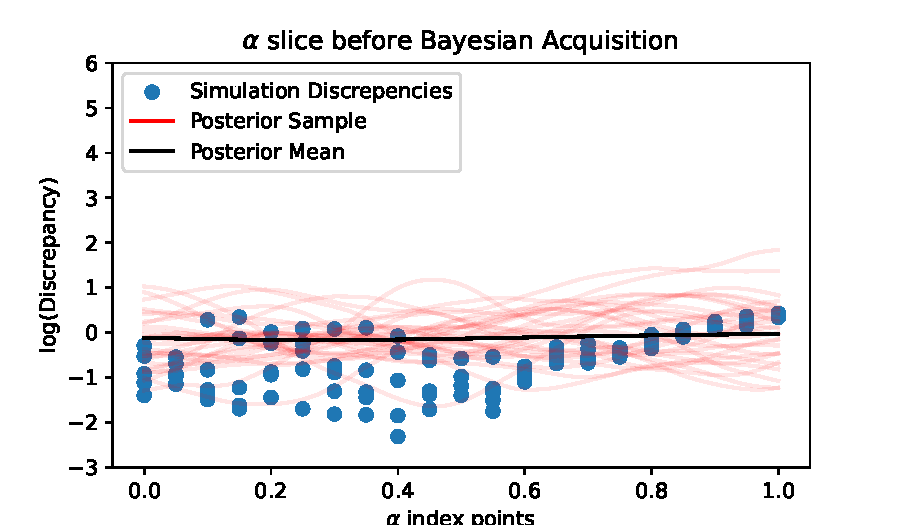
\includegraphics[width=\textwidth]{../champagne_GP_images/initial_alpha_slice_log_discrep.pdf}
    \end{subfigure}%
    \hfill%
    \begin{subfigure}[b]{0.33\textwidth}
        \centering
        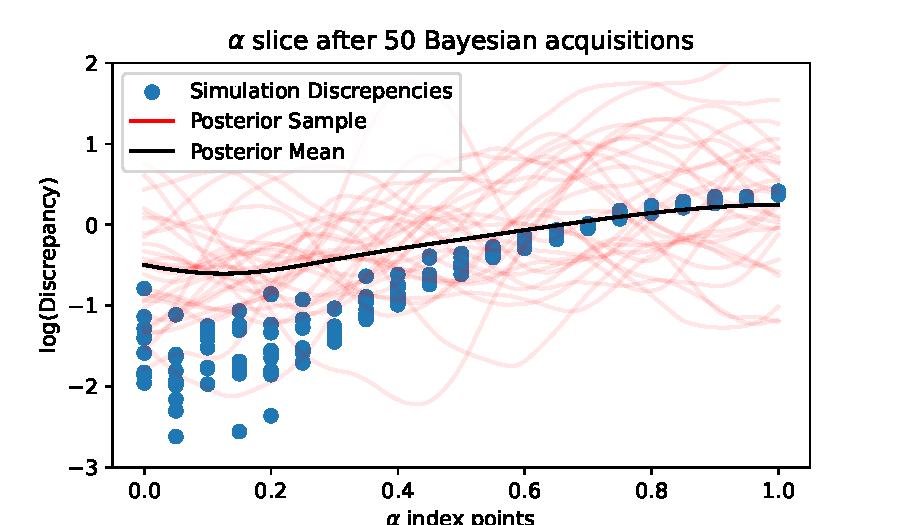
\includegraphics[width=\textwidth]{../champagne_GP_images/alpha_slice_50_bolfi_updates_log_discrep.pdf}
    \end{subfigure}
    \hfill%
    \begin{subfigure}[b]{0.33\textwidth}
        \centering
        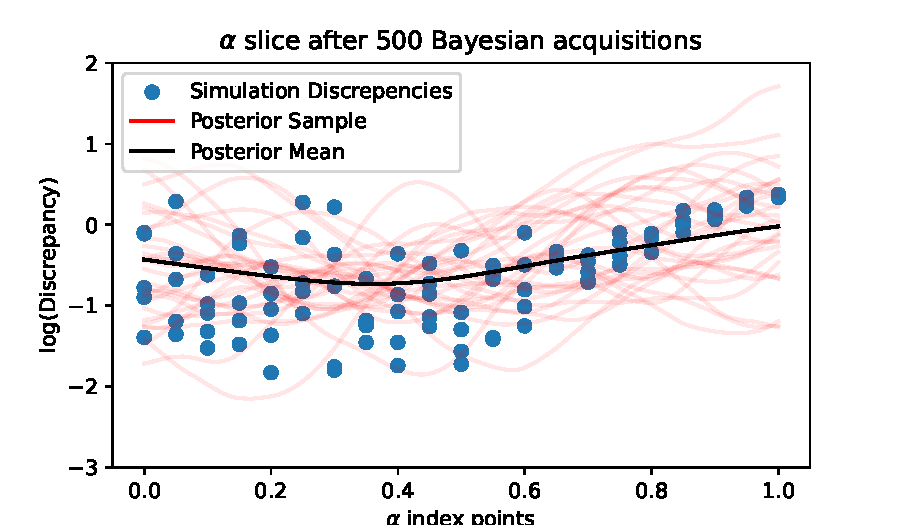
\includegraphics[width=\textwidth]{../champagne_GP_images/alpha_slice_500_bolfi_updates_log_discrep.pdf}
    \end{subfigure}
    \hfill%
    \begin{subfigure}[b]{0.33\textwidth}
        \centering
        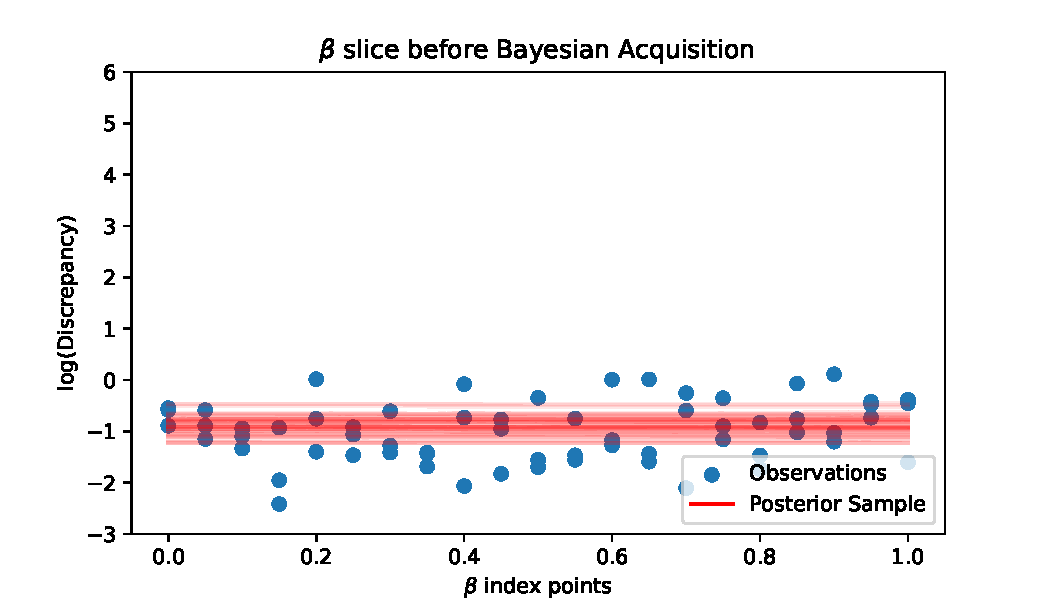
\includegraphics[width=\textwidth]{../champagne_GP_images/initial_beta_slice_log_discrep.pdf}
    \end{subfigure}%
    \hfill%
    \begin{subfigure}[b]{0.33\textwidth}
        \centering
        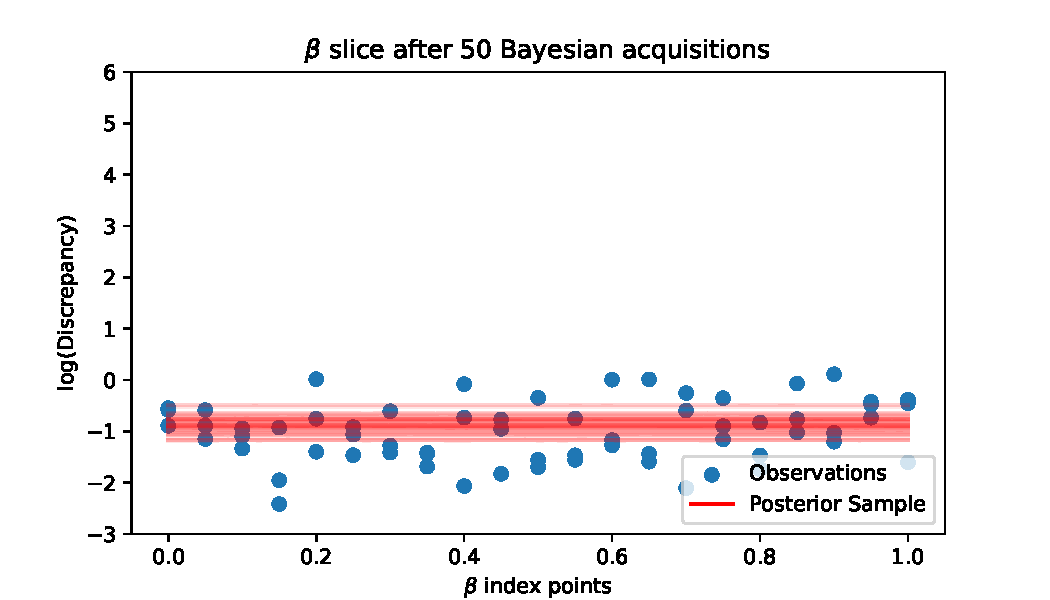
\includegraphics[width=\textwidth]{../champagne_GP_images/beta_slice_50_bolfi_updates_log_discrep.pdf}
    \end{subfigure}%
    \hfill%
    \begin{subfigure}[b]{0.33\textwidth}
        \centering
        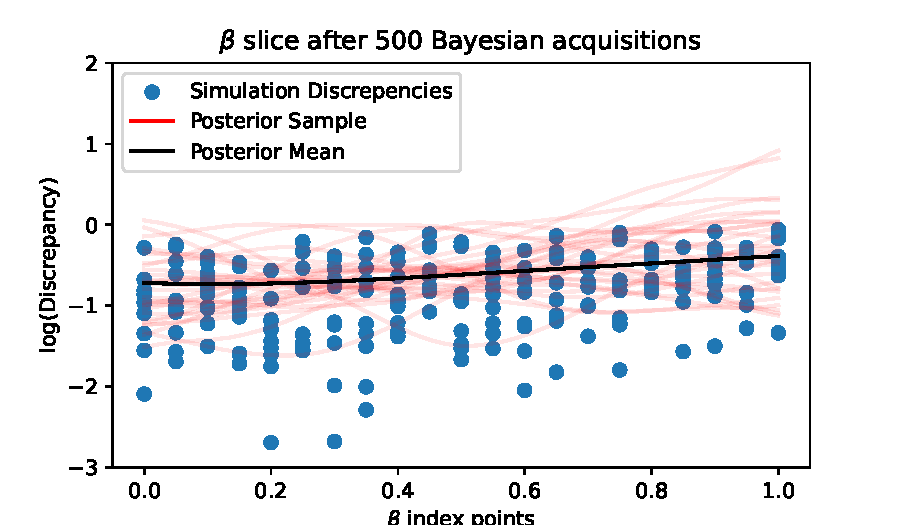
\includegraphics[width=\textwidth]{../champagne_GP_images/beta_slice_500_bolfi_updates_log_discrep.pdf}
    \end{subfigure}
    \begin{subfigure}[b]{0.33\textwidth}
        \centering
        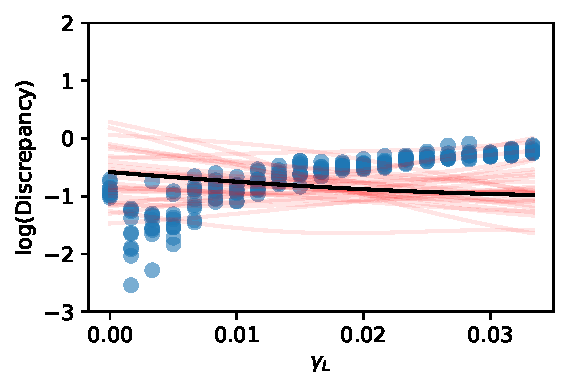
\includegraphics[width=\textwidth]{../champagne_GP_images/initial_gamma_L_slice_log_discrep.pdf}
    \end{subfigure}%
    \hfill%
    \begin{subfigure}[b]{0.33\textwidth}
        \centering
        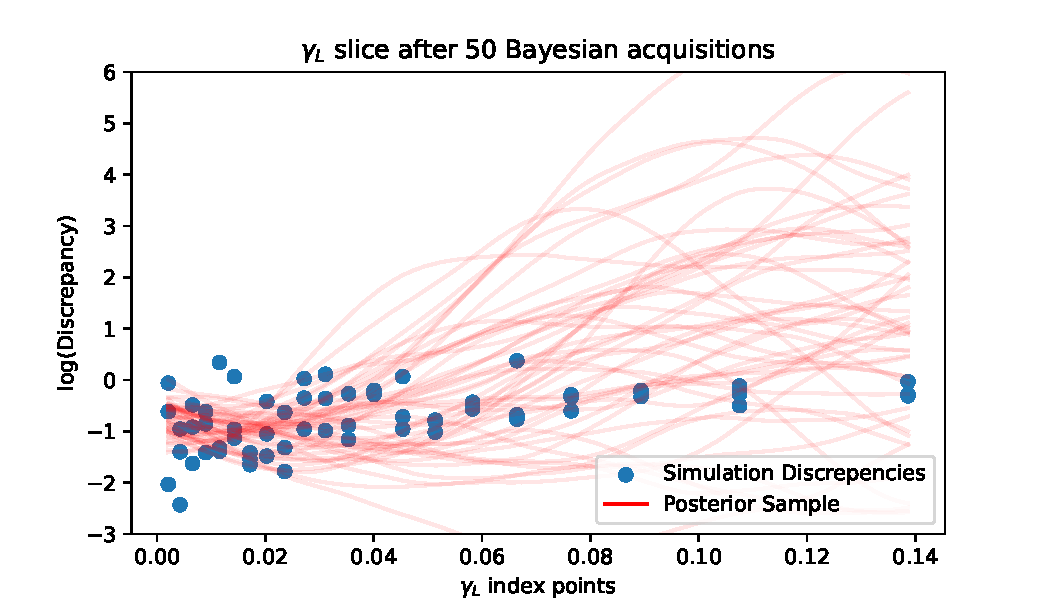
\includegraphics[width=\textwidth]{../champagne_GP_images/gamma_L_slice_50_bolfi_updates_log_discrep.pdf}
    \end{subfigure}%
    \hfill%
    \begin{subfigure}[b]{0.33\textwidth}
        \centering
        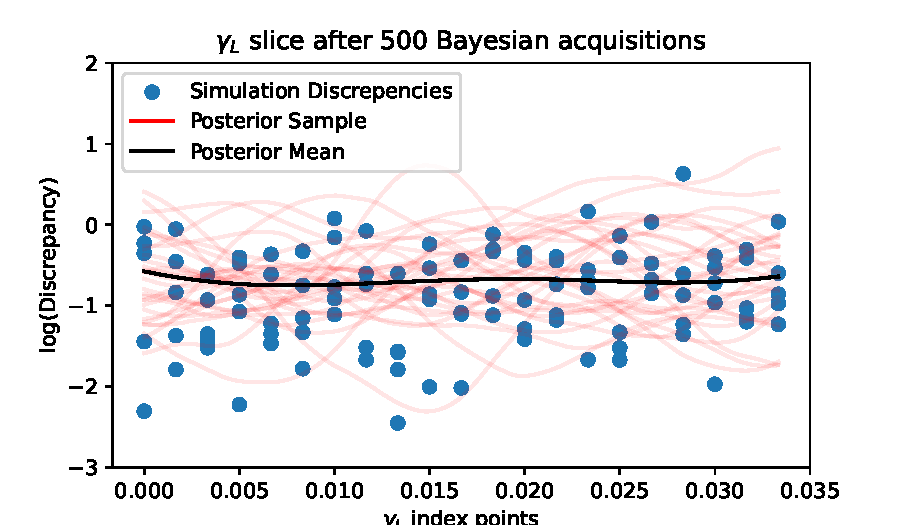
\includegraphics[width=\textwidth]{../champagne_GP_images/gamma_L_slice_500_bolfi_updates_log_discrep.pdf}
    \end{subfigure}
    \hfill%
    \begin{subfigure}[b]{0.33\textwidth}
        \centering
        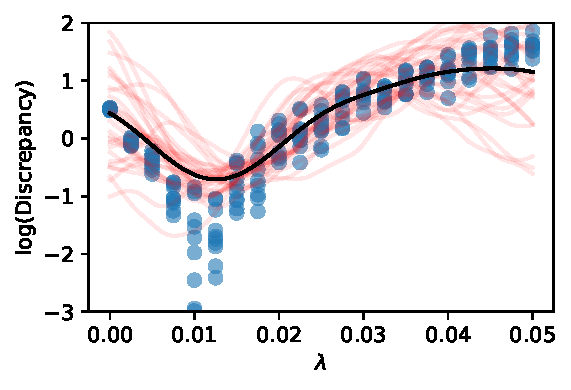
\includegraphics[width=\textwidth]{../champagne_GP_images/initial_lambda_slice_log_discrep.pdf}
    \end{subfigure}%
    \hfill%
    \begin{subfigure}[b]{0.33\textwidth}
        \centering
        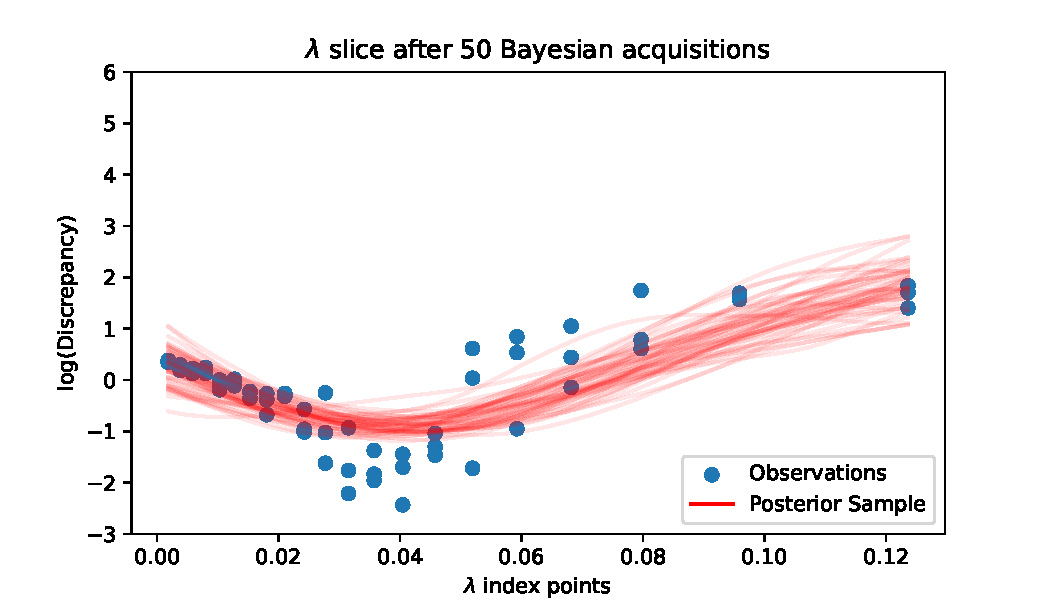
\includegraphics[width=\textwidth]{../champagne_GP_images/lambda_slice_50_bolfi_updates_log_discrep.pdf}
    \end{subfigure}%
    \hfill%
    \begin{subfigure}[b]{0.33\textwidth}
        \centering
        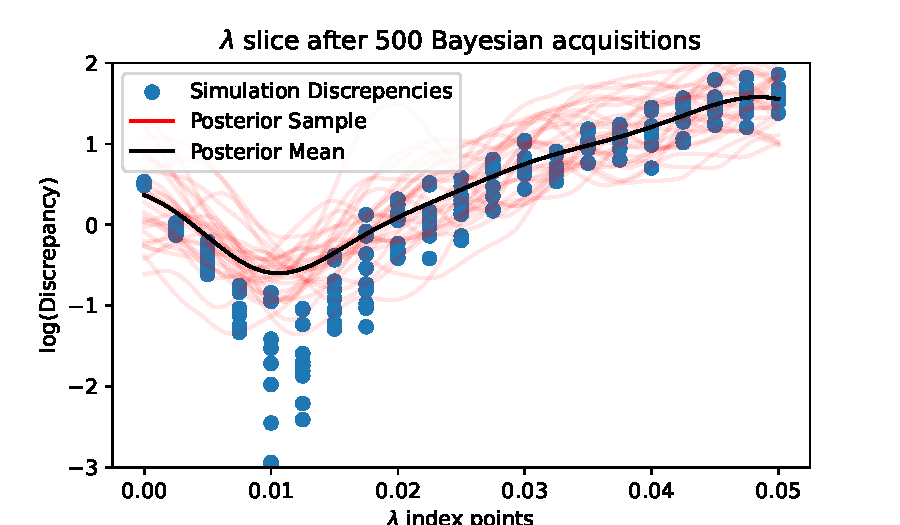
\includegraphics[width=\textwidth]{../champagne_GP_images/lambda_slice_500_bolfi_updates_log_discrep.pdf}
    \end{subfigure}
    \begin{subfigure}[b]{0.33\textwidth}
        \centering
        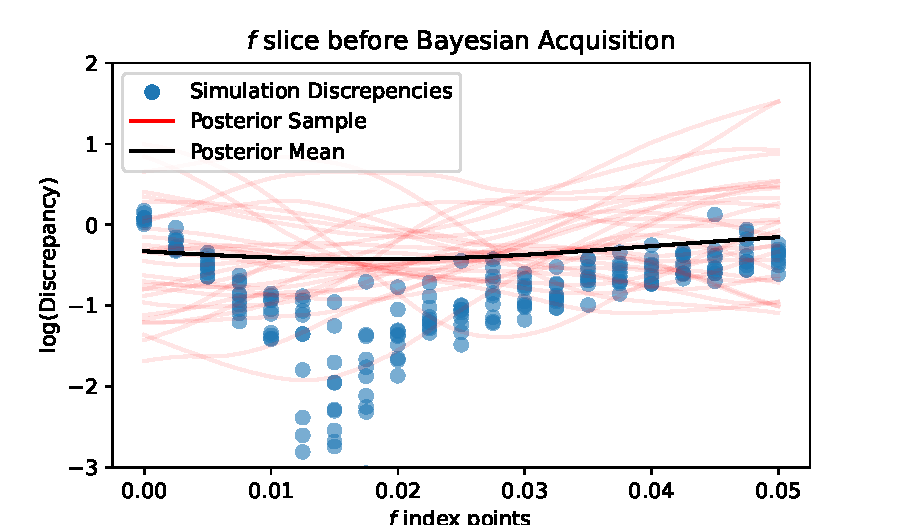
\includegraphics[width=\textwidth]{../champagne_GP_images/initial_f_slice_log_discrep.pdf}
    \end{subfigure}%
    \hfill%
    \begin{subfigure}[b]{0.33\textwidth}
        \centering
        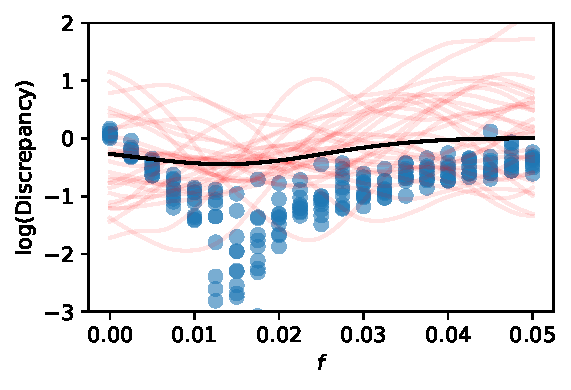
\includegraphics[width=\textwidth]{../champagne_GP_images/f_slice_50_bolfi_updates_log_discrep.pdf}
    \end{subfigure}%
    \hfill%
    \begin{subfigure}[b]{0.33\textwidth}
        \centering
        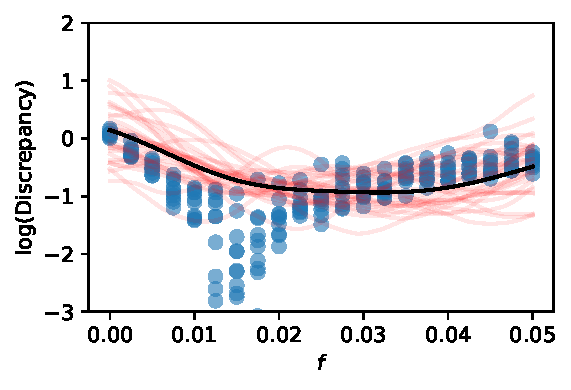
\includegraphics[width=\textwidth]{../champagne_GP_images/f_slice_500_bolfi_updates_log_discrep.pdf}
    \end{subfigure}
    \hfill%
    \begin{subfigure}[b]{0.33\textwidth}
        \centering
        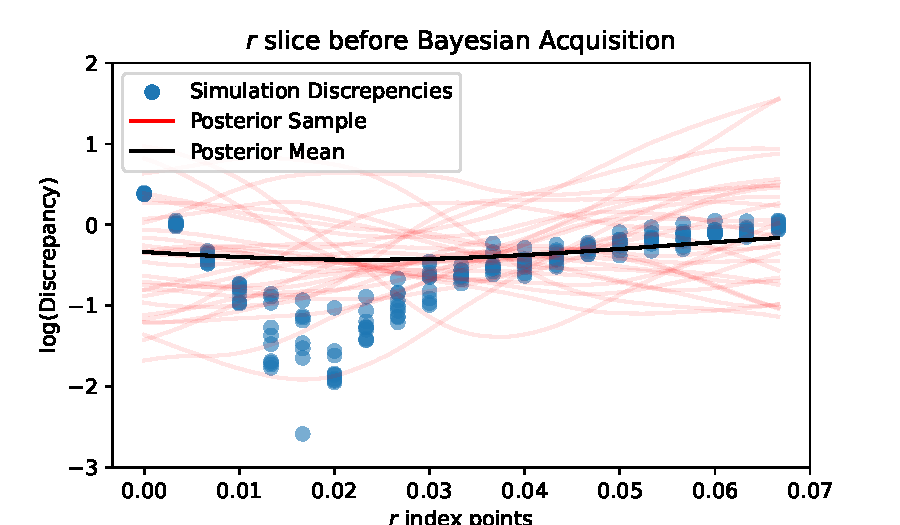
\includegraphics[width=\textwidth]{../champagne_GP_images/initial_r_slice_log_discrep.pdf}
    \end{subfigure}%
    \hfill%
    \begin{subfigure}[b]{0.33\textwidth}
        \centering
        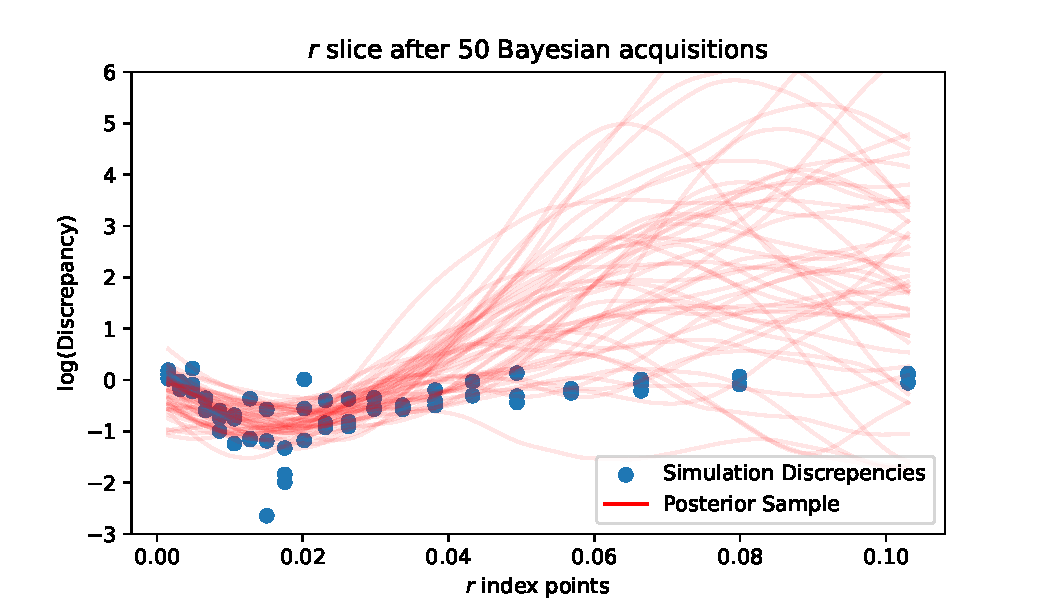
\includegraphics[width=\textwidth]{../champagne_GP_images/r_slice_50_bolfi_updates_log_discrep.pdf}
    \end{subfigure}%
    \hfill%
    \begin{subfigure}[b]{0.33\textwidth}
        \centering
        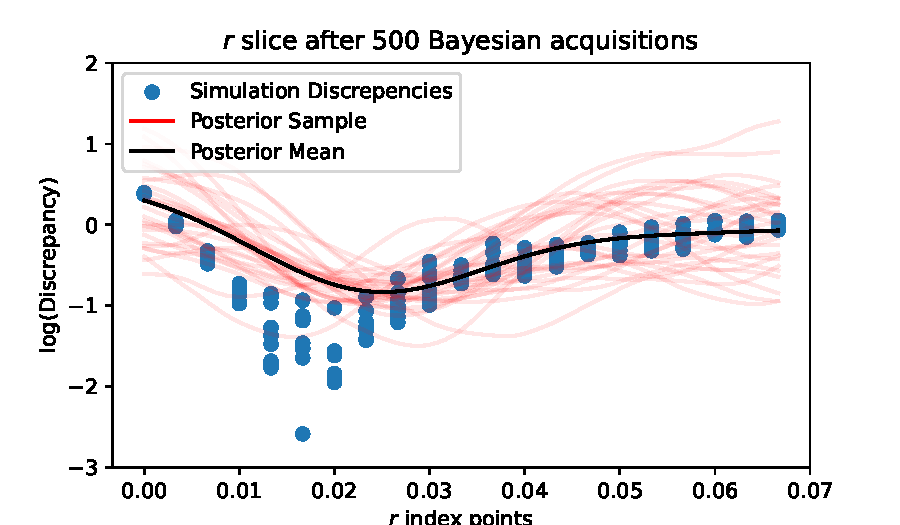
\includegraphics[width=\textwidth]{../champagne_GP_images/r_slice_500_bolfi_updates_log_discrep.pdf}
    \end{subfigure}
    \caption{
        Four sample discrepancies $\ln\mathcal{D}(\bm{\theta})$ taken along 21 
        values of each parameter to be predicted between the lower and upper 
        parameter bound.
        The Gaussian process predicts the mean of $\ln\mathcal{D}(\bm{\theta})$ 
        after initialisation, 
        50 iterations of Bayesian acquisition, and
        500 iterations of Bayesian acquisition.
        All parameters not in the slice are fixed at the true parameters that
        generated the synthetic observed data. The black lines are 
        $\E(d_\mathcal{GP}(\bm{\theta}))$ and the red lines are sample realisations
        from $(d_\mathcal{GP}(\bm{\theta}))$
    }
    \label{fig:improving_GP}
\end{figure}

As the number of Bayesian acquisitions increased, the Gaussian process mean 
seems to converge to the true mean, as seen in Figure \ref{fig:improving_GP}. 
The likelihood has maximum around the true values as seen in Figure
\ref{fig:final_synth_lik}. 
\textcolor{red}{I will add in lines where the true values are to this figure.}
There seems to be a lack of good data

\begin{figure}[htbp]
    \centering
    \begin{subfigure}[b]{0.5\textwidth}
        \centering
        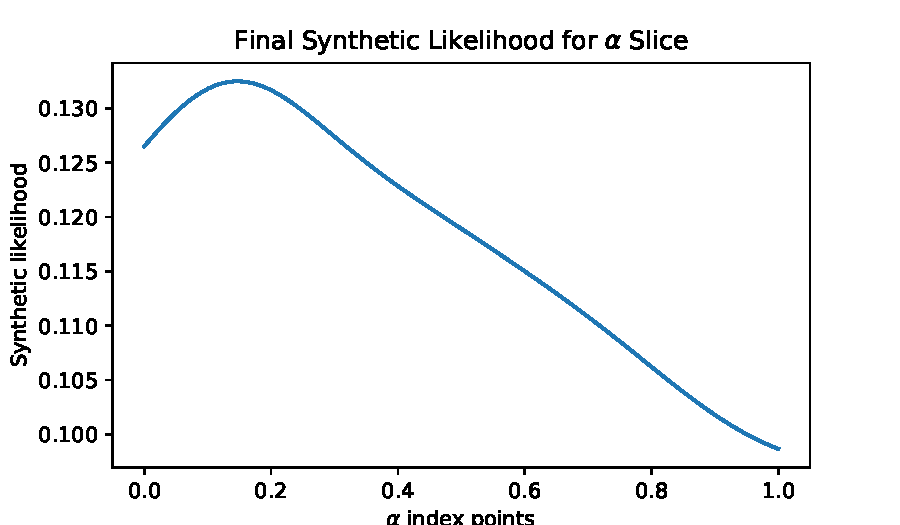
\includegraphics[width=\textwidth]{../champagne_GP_images/alpha_slice_500_synth_likelihood.pdf}
    \end{subfigure}%
    \hfill%
    \begin{subfigure}[b]{0.5\textwidth}
        \centering
        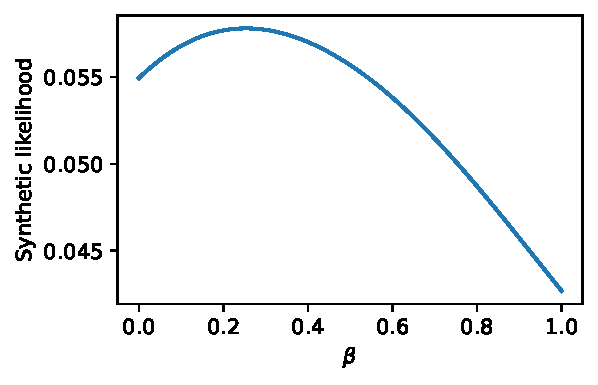
\includegraphics[width=\textwidth]{../champagne_GP_images/beta_slice_500_synth_likelihood.pdf}
    \end{subfigure}
    \begin{subfigure}[b]{0.5\textwidth}
        \centering
        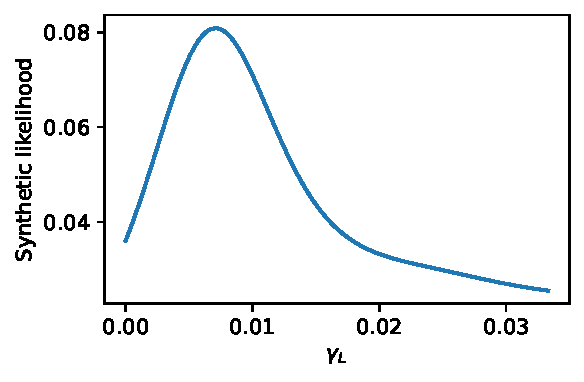
\includegraphics[width=\textwidth]{../champagne_GP_images/gamma_L_slice_500_synth_likelihood.pdf}
    \end{subfigure}%
    \hfill%
    \begin{subfigure}[b]{0.5\textwidth}
        \centering
        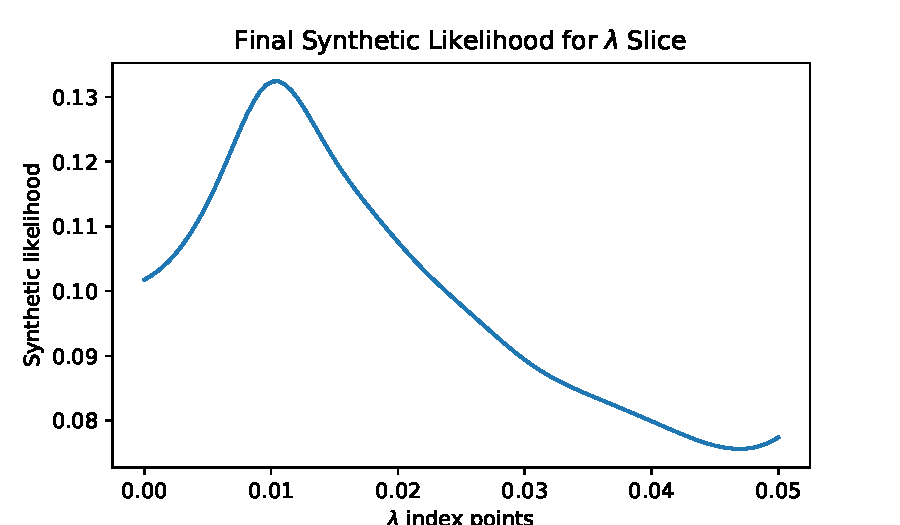
\includegraphics[width=\textwidth]{../champagne_GP_images/lambda_slice_500_synth_likelihood.pdf}
    \end{subfigure}
    \begin{subfigure}[b]{0.5\textwidth}
        \centering
        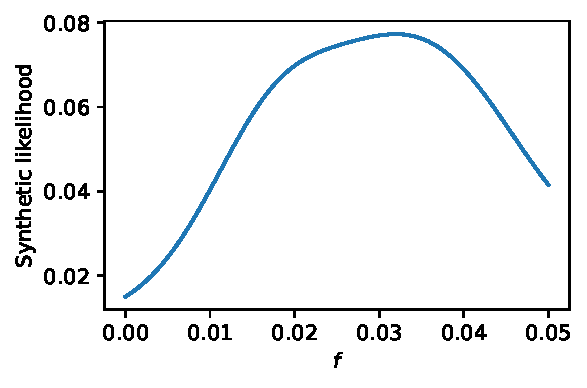
\includegraphics[width=\textwidth]{../champagne_GP_images/f_slice_500_synth_likelihood.pdf}
    \end{subfigure}%
    \hfill%
    \begin{subfigure}[b]{0.5\textwidth}
        \centering
        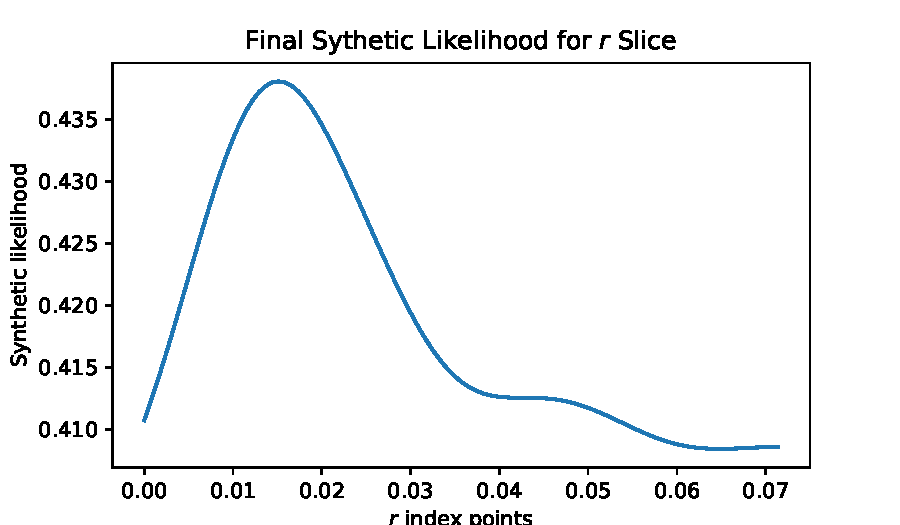
\includegraphics[width=\textwidth]{../champagne_GP_images/r_slice_500_synth_likelihood.pdf}
    \end{subfigure}%
    \caption{
        Final synthetic likelihoods $\hat{L}(\bm{\theta})$ after 500 iterations 
        of Bayesian acquisition. Each likelihood shows how that likelihood 
        changes across the parameter space.
    }
    \label{fig:final_synth_lik}
\end{figure}

\section{Discussion}

Although most of the procedure we used closely follows the paper by
\cite{gutmann_bayesian_2016}, there are a few key ways in which we modified the
manuscript's method. In particular, we felt the choice of squared exponential
kernel was not a good assumption, since it implicitly assumes a high degree of
smoothness in the target discrepency function. This is unlikely to be met if
the model has any bifurcation points. Under the squared exponential function,
if the true function has any sharp declines, or general non-smoothness
, the length scale is forced to be set very small. Therefore,
although the squared exponential is the most commonly chosen kernel,
we used a Mat\'ern kernel with $\nu = 5/2$. This is not as constrained as a
squared exponential kernel, but realisations are twice mean square
differentiable.

\cite{gutmann_bayesian_2016} use the lower confidence bound acquisition 
function, where the
exploration parameter is written as
$\eta_t:= \sqrt{2\ln(\frac{t^{2d + 2}\pi^2}{3\varepsilon})}.$ This seems to be
a mistake inherited from \cite{brochu_tutorial_2010}. Even using Brochu's 
original 
citation
\parencite{srinivas_gaussian_2010} to revise this to
$\eta_t:= \sqrt{2\ln(\frac{t^{2d + 2}\pi^2}{3\varepsilon})}.$
\footnote{One Python package that implements BOLFI notes this error, see:
    \url{
        https://github.com/elfi-dev/elfi/blob/dev/elfi/methods/bo/acquisition.py
    }
} When we tried both of these exploration parameters, the choice of 
$\varepsilon$ between $(0, 1)$ largely lead to repeated sampling from the same
set of parameters, even for very small $\varepsilon.$

This is problematic, as \cite{srinivas_gaussian_2010} assume a compact 
parameter space, whereas \cite{gutmann_bayesian_2016} do not.

They use a quadratic mean structure on unbounded parameters.
This could be problematic in situations 
where the discrepency has multiple local minima. When we tried it,
the quadratic mean function poorly it resulted in
in the acquisition function trying to sample extremely high parameter values.
Therefore we bounded our parameters, making out parameter space compact. 

\section{Further Work}

Moment matching could be used to avoid assuming that the distribution of 
the discrepency $\mathcal{D}(\bm{\theta})$ or $\ln\mathcal{D}(\bm{\theta})$ 
is normal for fixed $\mathcal{D}(\bm{\theta}).$ The sample variance could
be explicitly modelled using 